%%%% fatec-article.tex, 2024/03/10

\documentclass[
  a4paper,%% Tamanho de papel: a4paper, letterpaper (^), etc.
  12pt,%% Tamanho de fonte: 10pt (^), 11pt, 12pt, etc.
  english,%% Idioma secundário (penúltimo) (>)
  brazilian,%% Idioma primário (último) (>)
]{article}

%% Pacotes utilizados
\usepackage[]{fatec-article}
\usepackage{float}

%% Início do documento
\begin{document}
\vspace{8cm}
\begin{center}
    \large \textbf{\title{ARTEFATOS DO PROJETO DE SOFTWARE}}
\end{center}

\maketitle

\break

\tableofcontents

\break


%exemplo da forma de organização das seções e subseções, você deverá adaptar o template para a realidade do seu projeto.

\section*{Diagramas UML}
    Nesta seção serão apresentados os diagramas da UML utilizados para a modelagem do sistema desenvolvido. Dentre os diagramas utilizados, pode-se citar: Diagrama de Caso de Uso, Diagrama de Classe e Diagrama de Objetos.
    
    \subsection*{Diagrama de Caso de Uso}
    \addcontentsline{toc}{section}{Diagrama de Caso de Uso}

    Esse é um exemplo de diagrama de caso de uso, você deverá descrever todos os componentes presentes no diagrama (atores e funcionalidades do sistema).

\begin{figure}[H]
\centering
\caption{Diagrama de caso de uso}%
\label{fig:caso-de-uso}
 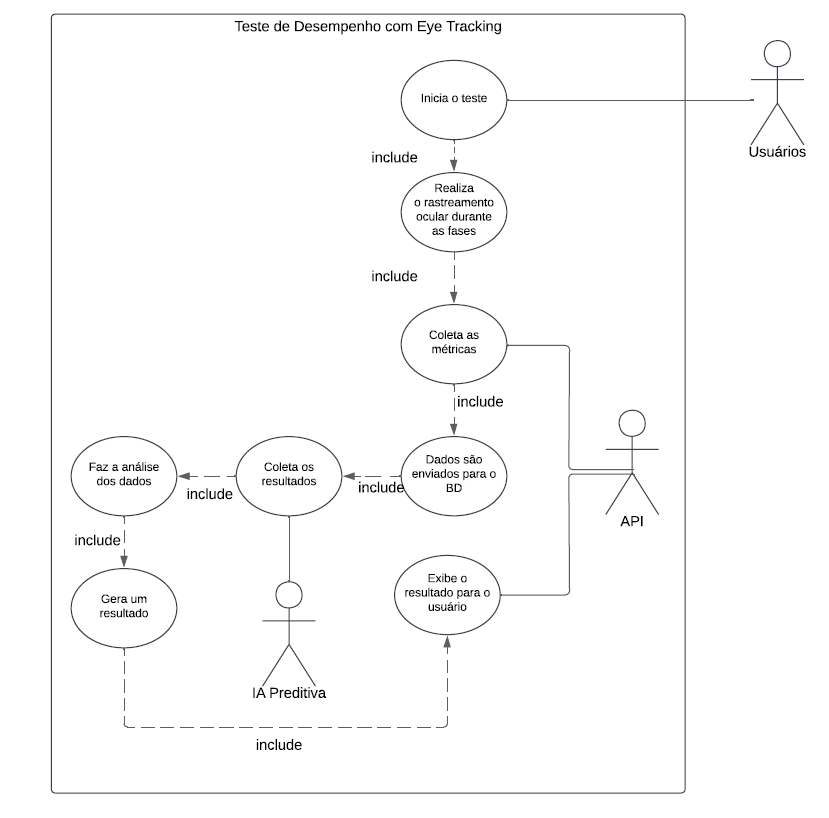
\includegraphics[width=1.1\textwidth]{Logos/caso-de-uso.png}
\SourceOrNote{Do próprio autor (2025)}
\end{figure}
    
    \subsection*{Diagrama de Classe}
    \addcontentsline{toc}{section}{Diagrama de Classe}

    Este Diagrama de Classe modela a estrutura de dados e as principais entidades do sistema de rastreamento ocular para avaliação de atenção.
    O diagrama ilustra quatro classes principais: Usuário, que armazena dados básicos de identificação, como nome, idade e sexo, além disso, contém os métodos logar(), logout(), jogar() e visualizarPréDiagnóstico(). A classe denominada Fases, que define as carcterísticas de cada fase do jogo, incluindo atributos como nome da fase (podendo variar entre "Fase 1", "Fase 2" e "Fase 3"), descrição, tempoTotal e o tipoAtençãoAvaliada. O método para esta classe é o iniciar() para começar uma fase do jogo. Possui a classe de Inteligência Aritifical (IA), que armazena os resultados brutos do rastreamento ocular, como dataTeste, usuário, métricas de foco (TempoInícioFoco, tempoMínimoFoco, tempoTotal, acertos), e contagens de erros (errosPorOmissão, errosPorComissão) todos como inteiros. A IA é responsável pelo processamento dos resultados e diagnóstico através dos métodos analisarResultados() e gerarPréDiagnóstico(). Por fim, a classe PréDiagnóstico que guarda o resultado final da avaliação de atenção para um usuário em uma determinada fase, incluindo usuário, fase, comentário e um valor de precisão. O pré diagnóstico é exibido ao usuário através do método mostrarPréDiagnósticoUsuário().

    \begin{figure}[H]
\centering
\caption{Diagrama de classe}%
\label{fig:diagrama-de-classe}
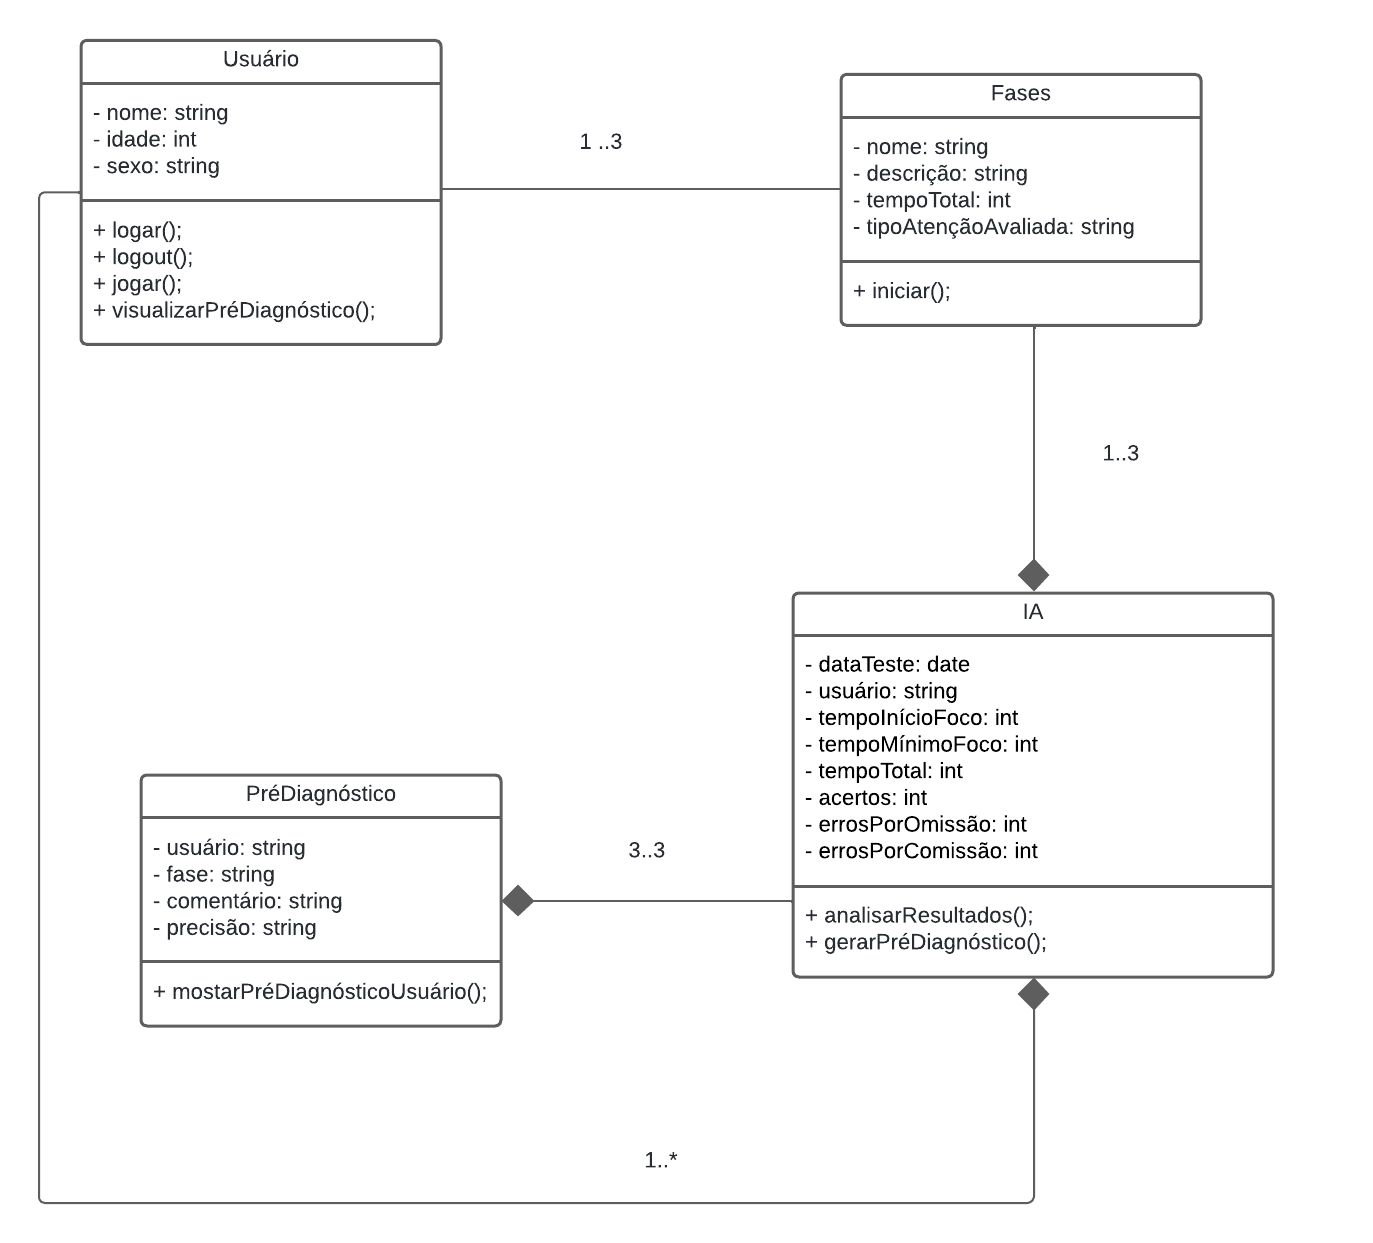
\includegraphics[width=0.8\textwidth]{Logos/diagrama-de-classe.png}
\SourceOrNote{Do próprio autor (2025)}
\end{figure}

    O diagrama de classe estabelece as seguintes associações e composições entre as classes: O relacionamente entre Usuário e Fases possui uma cardinalidade de uma para três, indicando que um usuário pode participar de até três fases do jogo. De forma semelhante, a associação entre Fases e IA também é de uma para três, refletindo que cada fase gera um conjunto de dados de rastreamento ocular. A classe IA está associada à classe PréDiagnóstico em uma relação de três para três, indicando que cada conjunto a IA pode gerar no mínimo e no máximo três pré diagnósticos, pois é um para cada fase do jogo. Por fim, a composição entre Usuário e PréDiagnóstico é de um para muitos, indicando que um usuário pode ter múltiplos pré diagnósticos ao longo do tempo.

    \subsection*{Diagrama de Objetos}
    \addcontentsline{toc}{section}{Diagrama de Objetos}

    O Diagrama de Objetos representa uma instância específica do sistema em execução, ilustrando os objetos concretos e seus relacionamentos em um determinado momento. Este diagrama exemplifica um cenário real do jogo, onde um usuário específico, identificado como "Manuela Santos", de 10 anos e sexo feminino, interage com uma das fases do sistema de avaliação de atenção.
    
    A instância do usuário está associada a um objeto de fase específico, denominada Fase 1, onde deve-se manter o olhar em cinco estrelas por 5s em cada com o tempo total de 60s e, que avalia a "Atenção Sustentada".
    
    Para esta fase executada, o sistema gera uma instância da classe IA contendo as métricas coletadas durante o rastreamento ocular, armazenando dados como tempo de início de foco, tempo mínimo de foco, tempo total, quantidade de acertos, erros por omissão e erros por comissão. Com base nesses dados, o sistema gera uma instância de pré-diagnóstico, associada à fase executada e contendo o comentário avaliativo "Atenção dentro do esperado", juntamente com o valor de precisão do olhar capturado.
    
    \begin{figure}[H]
\centering
\caption{Diagrama de objetos}%
\label{fig:diagrama-de-objetos}
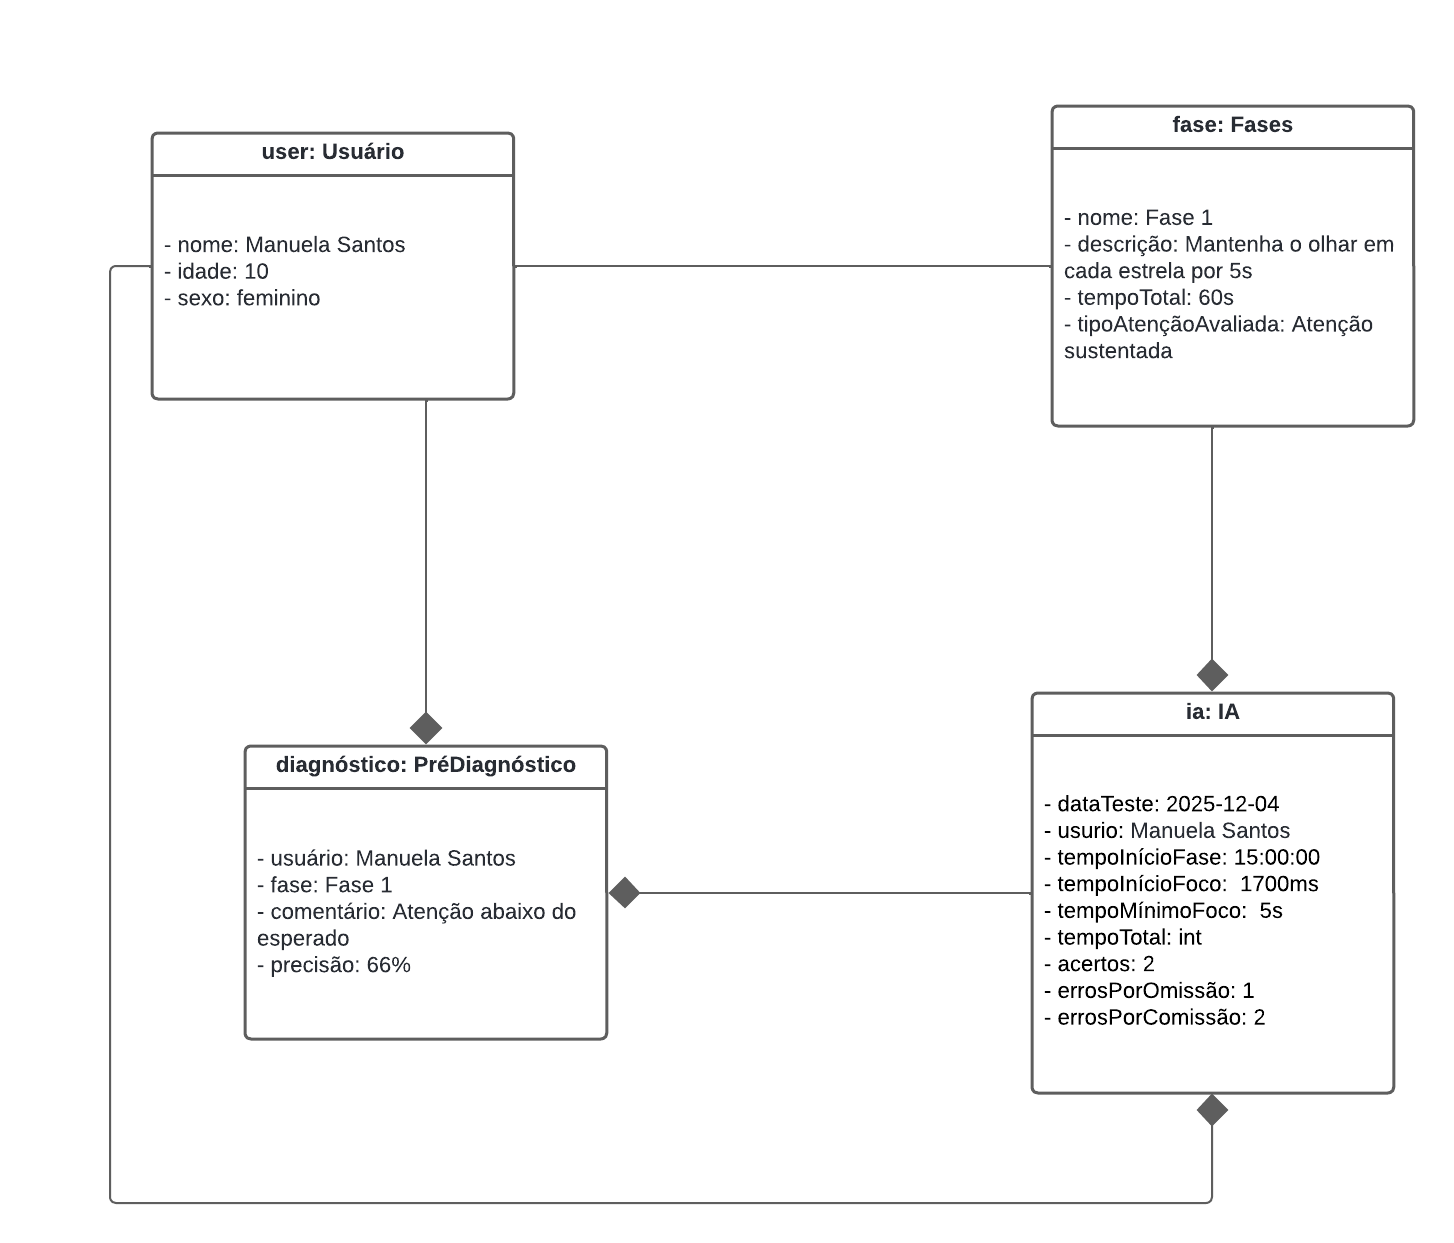
\includegraphics[width=0.8\textwidth]{Logos/diagrama-de-objetos.png}
\SourceOrNote{Do próprio autor (2025)}
\end{figure}

    Este diagrama ilustra concretamente como os dados fluem desde a interação do usuário com uma fase do jogo até a geração do pré-diagnóstico individualizado, demonstrando a aplicação prática da estrutura modelada no Diagrama de Classes através de uma instância específica do sistema.


\section*{Canavs}
    \addcontentsline{toc}{section}{Canvas}
    
    Esse é um exemplo de diagrama de redes, você deverá descrever todos os componentes presentes no diagrama (atores e funcionalidades do sistema).

\begin{figure}[H]
\centering
\caption{Canvas}%
\label{fig:canvas}
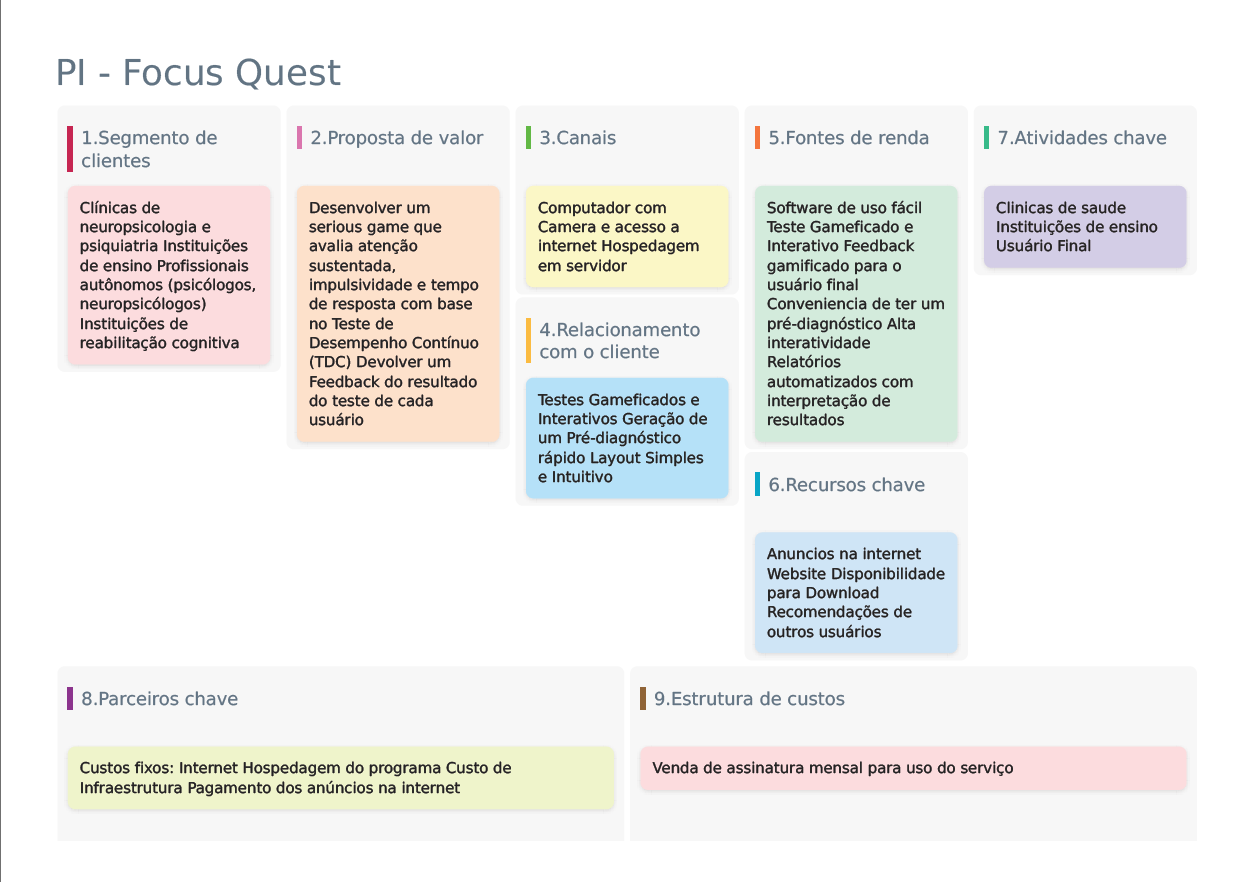
\includegraphics[width=1.1\textwidth]{Logos/canvas.png}
\SourceOrNote{Do próprio autor (2025)}
\end{figure}

    Não deixe a seção terminar com a imagem então sempre adicione um texto após a mesma.

\section*{Diagrama de redes}
    \addcontentsline{toc}{section}{Diagrama de Redes}
    
    Esse é um exemplo de diagrama de redes, você deverá descrever todos os componentes presentes no diagrama (atores e funcionalidades do sistema).

\begin{figure}[H]
\centering
\caption{Diagrama de redes}%
\label{fig:diagrama-de-redes}
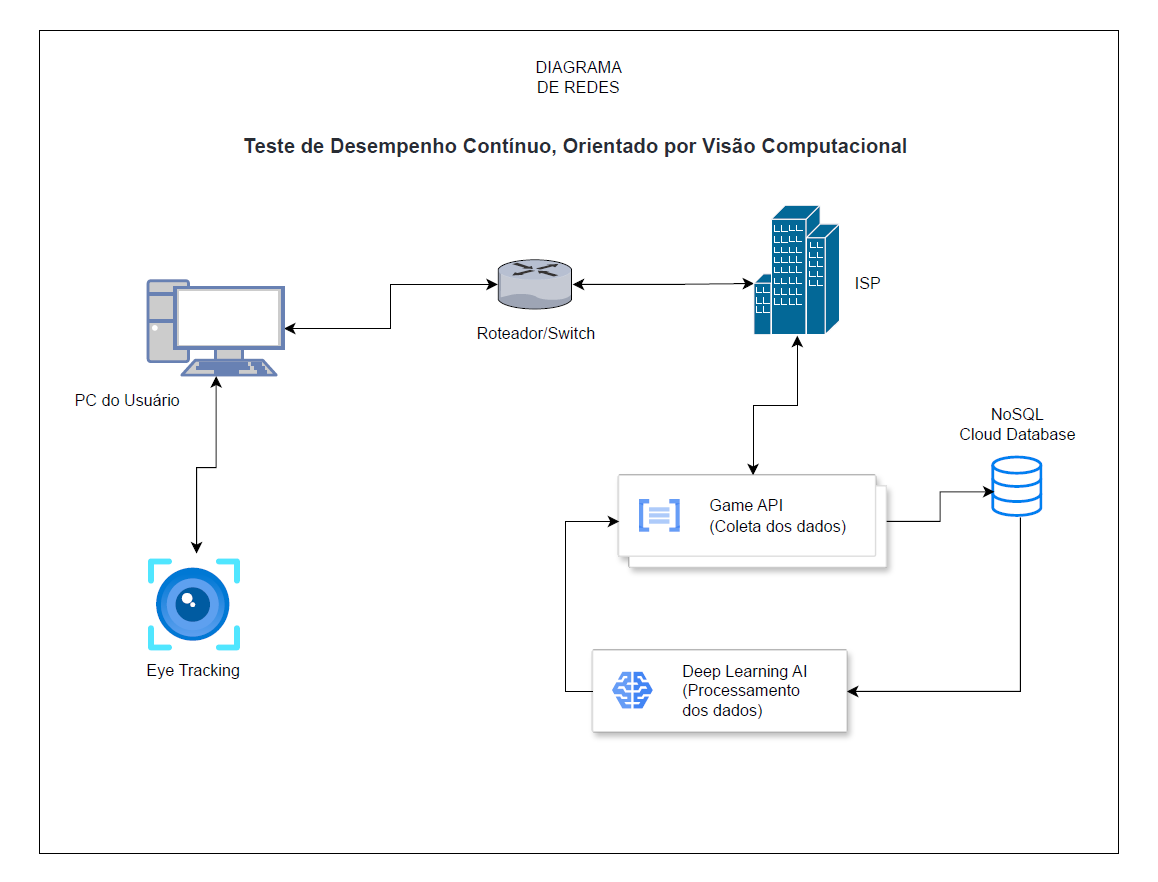
\includegraphics[width=1.1\textwidth]{Logos/diagrama-de-redes.png}
\SourceOrNote{Do próprio autor (2025)}
\end{figure}

    Não deixe a seção terminar com a imagem então sempre adicione um texto após a mesma.

\section*{Análise SWOT}
    \addcontentsline{toc}{section}{Análise SWOT}

    Esse é um exemplo de diagrama de redes, você deverá descrever todos os componentes presentes no diagrama (atores e funcionalidades do sistema).

\begin{figure}[H]
\centering
\caption{Análise SWOT}%
\label{fig:analise-swot}
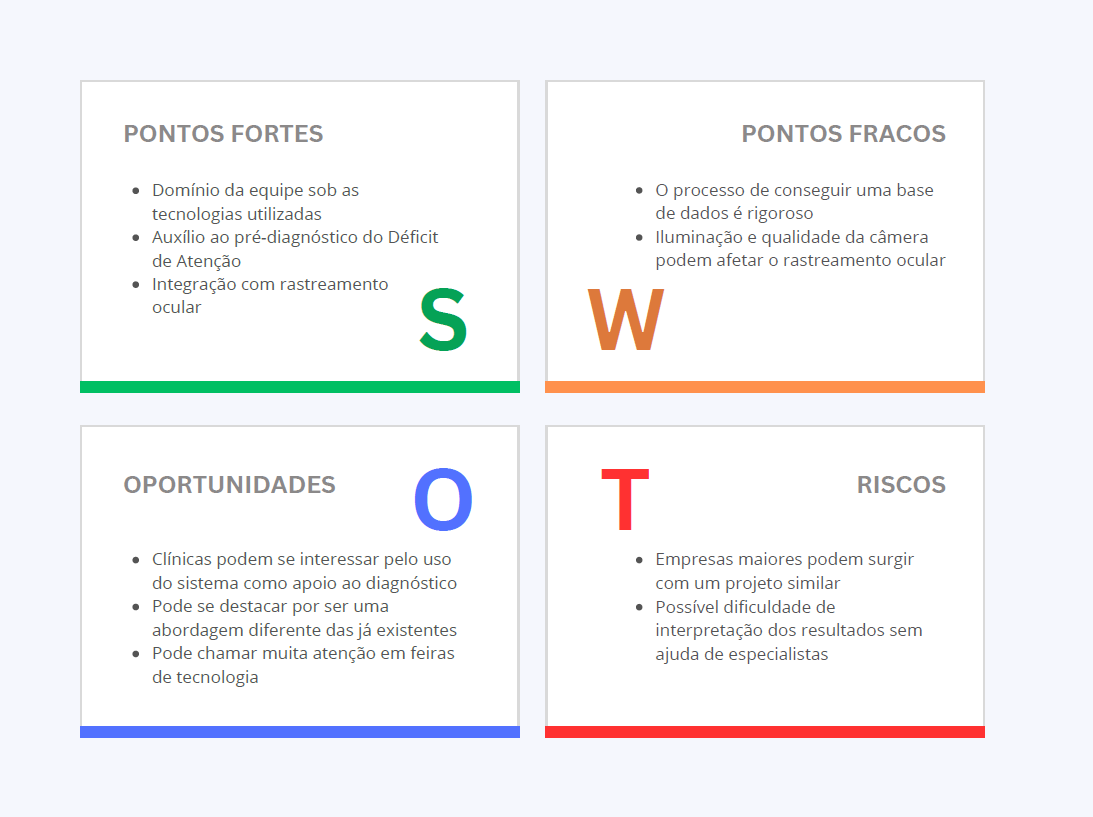
\includegraphics[width=1.1\textwidth]{Logos/swot.png}
\SourceOrNote{Do próprio autor (2025)}
\end{figure}

    Não deixe a seção terminar com a imagem então sempre adicione um texto após a mesma.

\end{document}

